\documentclass[a4paper]{article}
\usepackage[margin=1.2in]{geometry}
\usepackage{graphicx}
\usepackage{float}

\title{Blockchain-Based Auction Management}
\author{Filipe Pires (85122) \& João Alegria (85048)}
\date{\today}

\begin{document}
\maketitle

\begin{abstract}
This document describes the details of the development of an auction management system implemented with high security features.

The project was developed with the intent of studying several security mechanisms with great emphasis on the blockchain technology.

The resulting product allows for the users to manage auctions, make bids and validate results using their citizen cards for authentication and a command-line interface to interact with the program.
\end{abstract}

\section{Introduction} %%%%%%%%%%%%%%%%%%%%%%%%%%%%%%%%%%%%%%%%%%%%%
\label{sec:introduction}

The initiative for developing the Auction Management System (AMS) began with a proposal made by professors João Paulo Barraca and Vítor Cunha for the discipline of 'Segurança Informática e nas Organizações'.
The objective was to develop a software enabling users to create and participate in auctions protected by security mechanisms discussed during the semester.

The basic structure of the program is as follows. 
There are three main entities: an auction manager, an auction repository and auction clients. 
Their tasks are described in the second chapter of this document, as well as their implementations.
The software was designed to support four main security features: bids’ confidentiality, integrity and authentication, bid acceptance control and confirmation, bid author identity and anonymity and finally honesty assurance. 
These will also be explained further ahead, as they are present throughout the third chapter.

The messaging system is composed of two main sheds: multiple client-interfaces, through which users interact, and two servers, which serve as rendezvous points for all clients to connect. 
All messages are in JSON format, due to its user-friendly nature, and protected with a hybrid encryption.
The protection of the communication channels is also detailed in the third chapter.

\newpage
\section{System Entities} %%%%%%%%%%%%%%%%%%%%%%%%%%%%%%%%%%%%%%%%%%%%%
\label{sec:systementities}

In this chapter we will explain in detail the interacting entities of the system and present a high-level visualization of the architecture of the final result.

\subsection{Auction Client}

An auction client is an application that interacts with a user, enabling them to create and participate in auctions. 
The client's interface runs on a terminal (command-line interface).
This application needs to interact with the user Citizen Card (CC) in order to authenticate auction creation/termination requests or bids, therefore the user must have a smartcard reader connected to his host machine and to his CC in order to be able to use the software - see subsection \ref{subsec:authoridentification} for more information about this.

For each bid added to an auction, the auction client stores its receipt in non-volatile memory for an 'a posteriori' validation. 
This is fundamental for preventing both servers (described ahead) from cheating by manipulating the sequence of bids in a auction.

\begin{figure}[H]
\centering
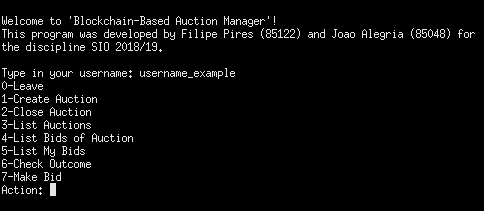
\includegraphics[width=0.8\linewidth]{UI.png}
\caption{Screenshot of the user interface menu.}
\label{fig:ui}
\end{figure}

The type of auctions proposed for this project are: 

\begin{itemize}
\item English Auction - a.k.a the Ascending Price Auction, characterized for each bid only being valid if it overcomes the value of the previous one. The user with the latest (highest) bid will be considered the winner and a new bidder receives the information about the current auction value before making his bid. The Auction Repository knows the user with the highest bid due to the nature of this auction type. The auction creator defines the lifetime of the auction, a minimum starting value, optionally limits the number of allowed bidders and allowed bids per user and may include python3-writen functions with specific formats for defining which kind of bids are accepted and which are not (validation function) and defining how will the process of subscription to that auction work (modification function) - see subsection \ref{subsec:dynamiccode} for more information about these functions. 
\item Blind Auction - a.k.a the Sealed First-Price Auction, characterized for no bidder knowing the current auction value (hence the name). The user with the highest bid will be considered the winner and a new bidder receives only the information about the auction's minimum value before making his bid. Once the auction is closed, the Auction Repository discovers the user with the highest bid. The auction creator defines the lifetime of the auction, a minimum value, optionally limits the number of allowed bidders and allowed bids per user and may include python3-writen validation and modification functions (like in the previous auction type). 
\end{itemize}

Aditionally, a new auction type was developed to improve the quality of the user experience. 
This auction type is called Reversed Auction and is described in subsection \ref{subsec:aditionalauctiontype}, since it is an extra feature of our system.

\subsection{Auction Manager}

This server exposes a connection endpoint through which clients can exchange structured requests/responses with it. 
The User communicates with the auction manager everytime he chooses to create or close an auction.
The manager is the system's entity that creates an auction upon the user's request. 
Upon such request, the manager instantiates a new auction in the auction repository. 
The same applies for the closing of an auction.

The auction manager is also the component that may perform special bid validations requested by the auction creator (the user). 
For instance, the auction creator may limit the number of bidders to a given set of identities, restrict the number of bids performed by each identity, etc. 
He may also define functions that control which bids are acceptable for his auction and which are not and control how does his auction's bid subscription work - such functions are performed by dynamic code uploaded to the Auction Manager at the time of the auction creation - see subsections \ref{subsec:dynamiccode} and \ref{subsec:bidvalidationandmanipulationfunctionsandsomeexamples} for more information about this.

\subsection{Auction Repository}

This server will expose a connection endpoint through which clients can exchange structured requests/responses with it. 
The user communicates with the auction repository everytime he chooses to: list auctions (active and closed), list all bids of an auction (only available once the auction has closed), list the user's bids on all auctions (only available those whose auctions have closed), find out the outcome of an auction and make a bid. 
To find out more information about how these actions work, see chapter \ref{sec:securitymechanisms}.

This component stores a list of auctions. 
Each auction is identified by a name, a unique serial number, a time limit for accepting new bids and a description. 
Each auction is implemented by a blockchain (a sequence of blocks were the last one ”seals” the previous sequence of blocks, making them immutable thereafter), with a bid per block. 
The repository closes an active auction upon a request made by the auction manager or upon reaching the auction’s time limit.

Users send new bids directly to the auction repository. 
The rate at which bids are sent is controlled by a mechanism called cryptopuzzle, or proof-of-work. 
A cryptopuzzle is a task that is hard to perform, while the result a such task is easy to validate. 
A client willing to send a bid first asks for a cryptopuzzle, then solves it, incorporates the solution in the bid and sends it to the repository. 
This, in return, checks the solution of the cryptopuzzle, optionally sends the bid to the auction manager to be validated, adds the bid to the auction blockchain and sends a receipt proving that the bid was added to the auction.

\begin{figure}[H]
\centering
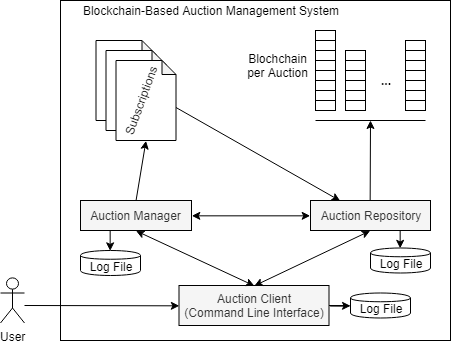
\includegraphics[width=0.65\linewidth]{SA.png}
\caption{High level architecture of the Auction Management System.}
\label{fig:sa}
\end{figure}

\newpage
\section{Security Mechanisms} %%%%%%%%%%%%%%%%%%%%%%%%%%%%%%%%%%%%%%%%%%%%%
\label{sec:securitymechanisms}

In the next chapters, we will use abreviations of the key terms of the report. 
Here are the direct translation of the abreviations:

Citizen Card - CC

Auction Client - AC

Auction Manager - AM

Auction Repository - AR

\subsection{Author Identification}
\label{subsec:authoridentification}

The first security mechanism lies on the side of the user. 
It is with a user authentication mechanism that the software assures the existence of a real person on the client end-point.

This authentication is achieved by the connection between the system's AC and a smartcard reader connected to the user's host machine with a valid CC inserted.
This is done with the help of the Python Library \emph{PyKCS11}.
All users are identified by a unique username (given to the AC once the program is running) that is intrinsically connected to the CC's public key, found in the smartcard's contents. 
This is crucial for the encryptions needed to communicate with the servers - see next subsection. 
The CC's private key is never seen by any entity. This characteristic is assured by the smartcard itself.

It is important to point out that the user must have possession of a letter containing the PINs to unlock the keys of authentication and digital signing. This usually comes with the CC.

During the development of this project, tested CCs were all in a valid state and belonged to real people.
We found that using ficticious CCs would not work as their certificate paths were incomplete and inconsistent.
It was also found that valid CCs older than 1 year have different paths and topologies, incompatible to our implementation - it is, therefore, recommended the use of recent CCs for the proper operation of the software.

\subsection{Message Protection}

As any system made for end users must be, ours is developed based on the assurance of secure communication channels and complete integrity of every message traded by all entities envolved.

Some of the reliable options for the communication channels were the following: TCP/IP, UDP/IP, HTTP, WebSockets, TLS.
Using WebSockets for the communication channels seemed to be a reliable choice, with the options of either TCP/IP or UDP/IP, or HTTP with a REST architecture, with the possibility of using security protocols such as TLS.
Our choice was of building WebSockets with TCP - since they would guarantee the message trading through unique communication tunnels, with simplicity and ease of implementation - and establish the security measures manually.
This does not mean that the other alternatives were worse, only that a choice had to be made. 

Regarding the security mechanism linked with the messages passed through the sockets' tunnels, we implemented a hybrid encryption approach. 
The encryption goes through 2 phases - the first one requires a symmetric key, and the second an asymmetric key-pair, hence the hybrid term.
All keys are generated from the file \emph{KeyGenerator.py} using the Python Library \emph{cryptography} that ensures the secure implementation of the cryptographic algorithms AES (for the symmetric key) with mode OFB and RSA (for the asymmetric key-pair). 
We chose these algorithms due to their cryptographic strength. 
The AES (Advanced Encryption Standard) algorithm is a block cipher standardized by NIST (National Institute of Standards and Technology), both fast and strong - tipically a good default choice for encryption. 
In our software, we use keys and IVs of size 32 and 16 bytes respectively.
The RSA algorithm (named after its authors R. Rivest, A. Shamir and L. Adleman) is one of the first public-key cryptosystems and is widely used for secure data transmission. 
Although slower than other algorithms, we found that its use would be appropriate since it would only be encrypting and decrypting the symmetric keys and not a large amount of bytes. 
Our system uses keys of size 512 bytes by default, but this value can be changed if desired.

The key generation functions inside the file \emph{KeyGenerator.py} store the keys in local files with names that follow a specific format.
Asymmetric keys are stored separately in files called \emph{entity\_private\_key.pem} and \emph{entity\_public\_key.pem}, where, in this case, \emph{entity} is replaced only by the name of the server entity to which the key belongs (i.e. manager or repository).
In the case of the users, asymmetric keys are generated by the program only for the communication and not for user authentication.
The authentification process is triggered when the user chooses a name to identify himself in the Auction Management System - here, the user's CC is crucial. 
This username must be unique and that condition is guaranteed by the AR; at the same time the user tries to find a valid name, the system identifies him as a person by asking him to sign his name. 
This signature is sent alongside the username and the CC certificate path, which gives the AR the suficient amount of information to validate the entire certificate path and the signature, fetching the public key from the person's signing certificate and verifying the signature provided. 
If all conditions meet, the user is accepted in the system and is given permission to enter in the main menu. 
From there on, every time a name appears in a request, if the system knows that name, it is assumed that that user is already authenticated.

\begin{figure}[H]
\centering
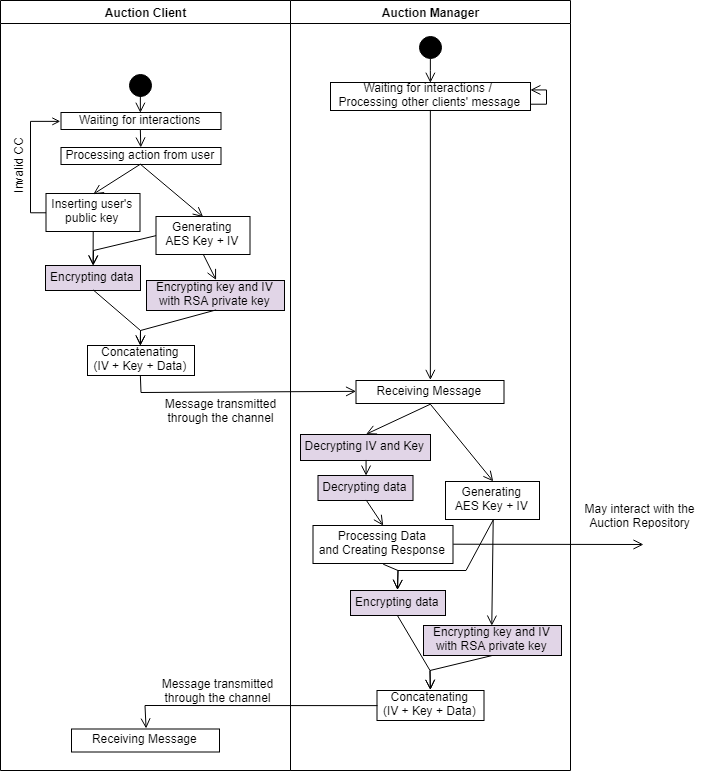
\includegraphics[width=0.9\linewidth]{ME.png}
\caption{Message exchange between an AC and the AM.}
\label{fig:me}
\end{figure}

Establishing a communication channel with the server implies the assumption that every user has access to and knows both the AM and AR's public keys.
The AC collects the data about the action that the user decides to execute, inserts the user's public key (generated when the AC is launched), generates a symmetric key and IV for the client and encrypts the data with them.
After this phase is completed, the AC encrypts the key and IV (previously generated) with the destination's public key (either the manager or the repository) separately and concatenates the 3 cryptograms with a specific delimiter known to the 3 entities of the system.
\newline The message is now ready to be sent.
Once the server receives it, it decrypts the user's symmetric key and IV with its private key and uses the decrypted content do decrypt the actual data.
After this, the server stores the user's public key for further secure communication with him.
To answer the user, the server creates the response data (e.g. action successfully executed) and follows the same process as the AC: encrypts the data with its symmetric key and IV, encrypts the key and IV with the user's now known public key, concatenates the 3 cryptograms with the same delimiter previously mentioned and sends the message through the communication channel.

All message trades follow this format.
The generation of asymmetric key-pairs is done once, before the system is booted. These keys must not change over time.
The server's private keys are stored with the code itself, meaning that if someone has access to them either the whole program is compromised and the attacker has access to the entire code as well as the keys, or that someone is the server itself.
The entities' symmetric keys are temporary and renewed everytime a new message must be sent.
Figure \ref{fig:me} helps understand the process of assuring the message confidentiality, representing in a visual and chronological format the processes related to the message exchange previously explained.

\subsection{Bid Protection \& Blockchain Construction}

The main concern of any user is the protection of the actions that envolve money and winning auctions - the bids.
Taking this in consideration, we reflected our main concerns with the users' and focused on assuring the correct manipulation of bids for each auction that the system hosts.
The general idea of how bids are dealt with and stored is as follows: all bids are sent by the AC to the AR, which runs a scan to verify them (regarding the integrity and validity of the bids), and inserts them into the list reserved for the auction to which each belongs; each auction therefore contains a list, and this list suffers from several operations that turn it into a fully encrypted and secure Blockchain.

When a user creates an auction, the AM verifies the validity of the validation / manipulation functions linked to the auction (if they exist), sends the information to the AR to be stored and keeps track of the development of the auction.
This is when the blockchain is created, storing in the first block all the metadata related to the auction: the name of the auction, the description, the timestamp of when it was created, the serial number, possible values for the minimum and margin restrictions and the dynamic code (if any).
Every block inserted afterwards consists of the content of a bid: the creation timestamp, the user, the amount, the auction and a checksum (using SHA256) value until the moment. 
The timestamp represents the instance of when the bid was accepted by the system.
The checksum value is the security mechanism that assures the integrity of the blockchain until the current block. 
This value is the result of the digest (using SHA256) operation over the previous block.

Each auction has the responsibility of creating its blockchain and updating it over time.
The AR is the coordinator of all auctions and keeps track of all "movements" recording them in a log file - see chapter \ref{subsec:logfile} for more information about this file.
The process of inserting a new block works as follows.
Assuming that the auction has already been created and the blockchain contains the first block with the auction's metadata, the first action of the auction is to generate the digest of the latest block and add it to the bid to be inserted.
After that, the bid is serialized and the first 16 bytes of the digest of the previous blocks are used as an IV for the encryption process.
Each auction contains a unique symmetric key generated by the auction also using the AES algorithm with mode OFB.
In the case of the first block, since there is no previous block to retrieve the first 16 bytes, the software uses the IV generated with the auction's symmetric key.
Now the server can encrypt the bid with the IV and unique auction key.
Once the encryption is completed, the auction executes an XOR operation over the cyphertext and the previously mentioned 16 bytes (or IV).
Since the XOR is a reversible operation, the decryption process will take advantage of this characteristic.
Each auction also has a blockchain sealing mechanism to prevent external users from being able to forge more blocks after receiving the entire blockchain and compromise the integrity of our system. 
\newline
This mechanism consists in when a auction ends, a new block is added in the end of the chain, block that has specific characteristics; it is a normal Bid object but it doesn't have amount nor user assigned to it while having the checksum (using SHA256) of the last block, since no one has submited it. The last detail that differentiates this last block from the remaining is that it is encrypted with the AR public, signifying that only the AR can decrypt this last block. The combination of the checksum and the different encryption makes sure the seal block can't be placed elsewhere in the chain, sealing it.
Finally the result is ready to be inserted in the blockchain.

The decryption process is explained in chapter \ref{subsec:bidexposureandauctionvalidation}.

\subsection{Cryptopuzzle Deployment}

Cryptopuzzles are an important asset to the Auction Management System since they help regulating the rate at which bids are sent by each user.
To better understand the regulation problem, lets analyse a use case: the Ebay's auction system.
It has been many years that Ebay began to host online auctions by any seller with an account to any buyer.
How it works is simple - the seller defines the rules of the auction, defines the expiration time and awaits for bidders to make their bids until the time is over.
However, what happens in these auctions is what is called \emph{sniping}, where a group of bidders await for the final seconds of the auction to make their bids and seal the victory. 
Not only does this give a false sense of the value of what is being sold during the auction, but also makes wining an auction a matter of luck and speed of Internet.
Here is where cryptopuzzles come in.
These tasks (more or less hard to perform) are placed upon bidders in order to force them to complete a puzzle if they desire to go through with a new bid.
As users have to take in consideration the time they spend to complete a bid, not only the number of attempts to somehow sabotage an auction decreases, but also the occurrence of sniping practically disappears.

The main characteristic of a well implemented cryptopuzzle is that it presents a challenge that requires a certain amount of time and effort to be solved.
In our case, the cryptopuzzle is a simple comparison of bytes. Here is how it works.
When a user decides to make a bid, he sends to the AR the auction that he is interested in.
Then, the AR produces X random bytes, where X is the number of bytes defined by the auction creator, with the help of the Python Library \emph{OS} and the cryptographically secure function \emph{urandom} - these bytes are sent as a challenge for the user along with the information about the current state of the auction, if available (current, margin and step values).
Once the AC receives the response, it presents the auction information to the user and awaits for the user to fill in the fields related to the bid.
As soon as the user finishes, the AC executes a process to find the solution to the challenge. 
This process consists of producing 16 random bytes and inserting them in the bid, then calculating the checksum (using SHA256) of the bid with those 16 bytes and comparing the first X bytes of the result with the challenge of the server.
If the bytes match, the AC has found the solution and so it stores the resulting bid in an auxiliar variable. If not, the AC removes the 16 bytes from the bid and repeats the process with new random bytes until a solution is found.
The level of difficulty defined by the auction creator will determine how long will it take for the AC to find the solution - the bigger the value of X, the lower are the chances of the AC finding out a solution quicly. 
This task is already a means of increasing the time needed to submit a new bid and therefore reduce the changes of the occurrence of the sniping effect.

In addition to this, we present to the user a task as well. 
After finding the solution, the AC inserts to an auxiliar list the first X bytes of the checksum found, along with several other first X bytes of other checksums that do not solve the puzzle.
Now, it starts to ask the user to compare an element of that list (in a random position) with the value of the puzzle.
If the user decides that the two do not match, the AC discards the element and repeats the process until the user finds the 2 matching elements (the solution).
Figure \ref{fig:cp} shows an example of a cryptopuzzle being solved by a user in the software's interface.

Completed the task, the AC sends the response to the AR, which decrypts the message, retrieves the bytes from the bid and verifies if the first X bytes of the checksum of the bid with those 16 bytes match the puzzle that it had sent before.
If so, it then proceeds to completing the bid execution, if not, the AR returns an error message explaining that the user failed the cryptopuzzle.

\begin{figure}[H]
\centering
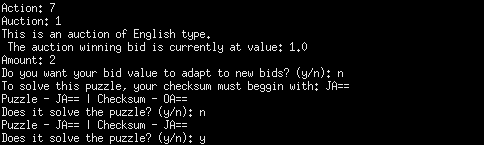
\includegraphics[width=0.8\linewidth]{CP.png}
\caption{Screenshot of the user interface cryptopuzzle filling.}
\label{fig:cp}
\end{figure}

Note: the cryptopuzzles are not useful only for situations such as ours; they many times require critical thinking for the challenge attempters who undoubtedly learn something new in the process of decoding them, so they can be used as games or forms of art.

\subsection{Dynamic Code: Bid Validation \& Valid Bid Modification}
\label{subsec:dynamiccode}

Allowing users to run code of their own during auctions is an exciting idea to many potential auction creators.
This is due to the freedom it gives to the user to filter bids and impose conditions to his auction the way he pleases.
However, the existance of dynamic code inside a program represents a challenge to any developer, since it opens doors to the abuse of power by the user.
Taking this into account, preventive and restrictive security mechanisms must be present in the part of the system that accepts external executable code.

Our Auction Management System supports two types of dynamic code - bid validation and valid bid modification - each delimited by a single function.
Users may give assign these two functions (or just one, or none) to an auction on creation by writing them in the AC interface according to a specific format.
Details about the format are present in chapter \ref{subsec:bidvalidationandmanipulationfunctionsandsomeexamples}.
In this section, we focus on the motive behind the implementation of such features, the type of operations that a user may include in such functions and how does the software deal with them in a secure and syncronous manner.

The validation function will be executed everytime a bid is sent to the AR and validated by the program as the final step to completely validate the bid. This step is ignored if the validation function is empty. 
The auction creator may apply conditions inside this function such as: preventing bidders from increasing the auction's current value in very low percentages, making calculations that may be of his interest (with limited scope), etc.

When a user makes a bid, he may choose to subscribe to that auction and define how much is he willing to pay - in this case, the modification function will be activated for him and a thread dedicated to the update of his bids will start.
The modification function will be executed by this thread everytime a bid is sent to the AR and completely validated by the server, if the new bid is not from the same user as the one linked to the thread (i.e. if the thread's original bidder isn't the one bidding). 
If the user decides to make a new subscription to the same auction, the previous thread reads the limits as usual (with the values now updated).
The auction creator may apply operations inside this function such as: defining what value will the new bid have, restricting the maximum value possible for subscriptions, etc.

An example of a validation and a modification function is present at the end of chapter \ref{subsec:bidvalidationandmanipulationfunctionsandsomeexamples}. More examples (including invalid ones) are present in the file called "ExampleFunctions.py".

More specific restrictions related to auctions are not included in the dynamic functions due to several reasons.
These details are: limit of the number of bidders allowed, limit of the number of bids performable by each bidder, level of difficulty of the cryptopuzzle (the value of X explained in the previous section).
We decided to make these auction fields only definable through the AC menu options because our intentions towards the dynamic code were not to make it mandatory and purpose specific but instead an opportunity for the user to personalize his auction.
As the reader may understand from the use case examples previously mentioned, our dynamic code functions allow the user to do just that in a controlled way.

\newpage
\subsection{Bid Exposure \& Auction Validation}
\label{subsec:bidexposureandauctionvalidation}

The concept of bid exposure appears when we view the program from the perspective of a sceptic user.
Such user would only make bids if he fully trusted the software.
The bid exposure is the security mechanism that allows the system to prove to any user that no corruption takes place during the auctions - by giving the bidder all that the server stores and the keys needed to decrypt and validate the content (if applied). 
Our Auction Management System makes available 2 sorts of bid exposure: the exposure of all information about a specific closed auction (excluding the private information about each bidder) and the exposure of all information about all bids made by the user that asks for it.
In this subsection we will discuss them individually.

The 4th option of the AC menu - \emph{List Bids of Auction} - allows a user to ask for an exposure of all the progress of a specific auction.
He reffers which auction he intends to inspect through the serial number and the only condition that the server imposes for the user to have the permission to see the content is that the auction must be closed.
For the server, each auction represents a blockchain, so in order to allow the user to verify the integrity of an auction and its outcome, the blockchain must be made available for the bidders along with the sufficient tools to extract the data in clear text.
Taking this in consideration, if the condition imposed by the server is true, the AR builds a response message containing 3 elements: the entire blockchain of the auction, the private symmetric auction key and IV.
Then, the AC presents these elements to the user and asks him if he desires to decrypt the blockchain and analyse the data.
This extra feature has the intention of making the decryption process easier for the user, however the user himself may take the information given and do the decryption on his own.
Chapter \ref{subsec:validatinganauction} explains how the user can do this.

The 5th option of the AC menu - \emph{List My Bids} - allows a user to ask for an exposure of all of his bids throughout the closed and opened auctions.
In this sort of bid exposure, the user does not need to give any information to the server.
However, this feature does not have the purpose of prooving the integrity of the auctions. 
Instead, it focuses on giving the chance for the user to verify that all his bids were actually considered by the server.
What the option does is asking the AR to build a response message containing all the bids made by the user and send it to the AC, which in return exposes the information to the user.
The AR here decrypts all auctions where the user participates and responds with the user's bids in plaintext, as for the owner no secret is kept.

\begin{figure}[H]
\centering
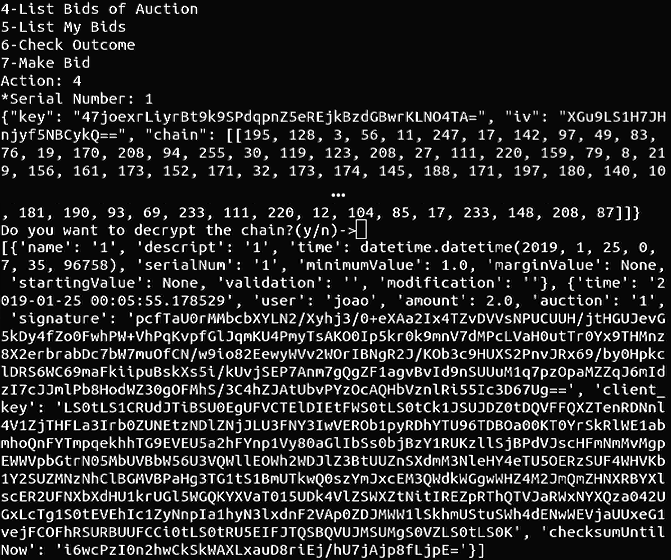
\includegraphics[width=0.7\linewidth]{BE.png}
\caption{Screenshot of exposure of a closed auction. Note: the blockchain is shortened for visualization purposes.}
\label{fig:be}
\end{figure}

\subsection{Bid Receipts}

When a user makes a bid, the software must be prepared to notify him whether the action was successfully executed or not and return some sort of proof.
The Auction Management System has a specific feature for that purpose - the bid receipt.
This receipt is a simple document with a signature of the server that is accepted as proof for the user that the operation has been completed.

Receipts are created by the AR when the system consolidates the users' bids. 
They are sent as response to the user in the same secure communication channel between the AR and AC.
A receipt is a JSON object containing the serial number of the auction, the username, the bid's amount and the evidence of the operation's completion.
It is important to mention that the way the communication channel is built is enough to ensure that the receipt was created by the AR.
However, we decided to include a signature inside the receipt as an extra security measure and a more direct proof for the user that reads the receipt.
This signature is basically the name of the bid's owner signed by the AR.

If the user desires to confirm that the signature is of the server, he simply needs to use the AR's public key to verify whether if it was the one signing the value or not (with the help of the \emph{Cryptography} library's funtion \emph{public\_key.verify()}.
Still, the AC makes this verification on his own and gives the result to the user as well.

\begin{figure}[H]
\centering
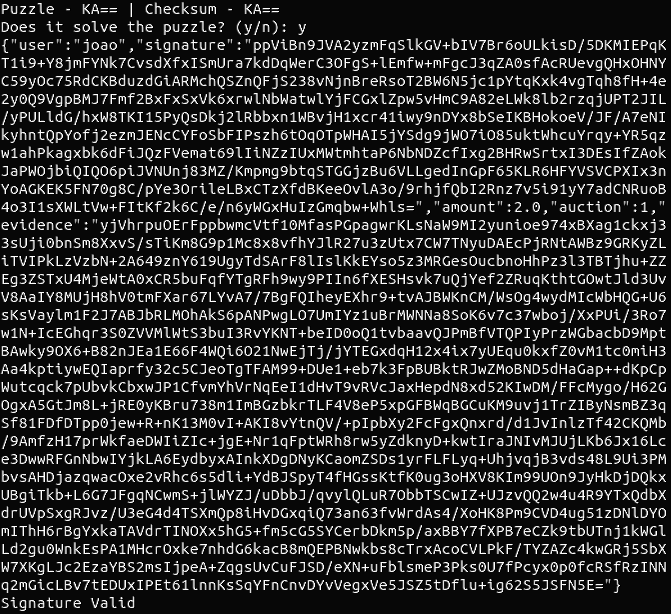
\includegraphics[width=0.8\linewidth]{BR.png}
\caption{Screenshot of a bid receipt once the bid is accepted. Note: the final line shows the signature validation made by the system itself.}
\label{fig:br}
\end{figure}

\newpage
\section{Aditional Information} %%%%%%%%%%%%%%%%%%%%%%%%%%%%%%%%%%%%%%%%%%%%%
\label{sec:aditionalinformation}

This chapter displays information about details of the project concerning: how to deploy the program, how to manually validate an auction, how does the key-pair generation work, which are the implementation's problems and where are its weaknesses, what aditional features were introduced. Some code examples for the bid validation and manipulation functions are also available at the end of this chapter.

It is important to point out that all code developed during this project is available at the git repository (link available in the next subsection), including auxiliary scripts and example functions.

\subsection{Deployment}

In order to completely deploy the Auction Management System, a person must have:
\begin{enumerate}
\item Linux OS or VM (may work with other OS such as Windows but requires changes to the deployment script)
\item Python 3.6 installed (older versions may work but no guarantees are given)
\item Python PKCS11 module installed
\item Docker Platform installed
\item Smartcard Reader and up-to-date Citizen Card
\end{enumerate}

The project's code is available at: https://code.ua.pt/git/sio2018-p1g8.
Once all requirements are assured and the git repository is downloaded (warning: link may change after this document is published), a person needs to:
\begin{itemize}
\item Enter the project's folder:

\indent \$ cd sio2018-p1g8

\item Create a network for the system and the AR's docker image:

\indent \$ docker network create --subnet=172.18.0.0/16 sio

\indent \$ docker build -t repo .

\item Alter the dockerfile to create the AM's docker image:

\indent \$ nano Dockerfile

\indent [comment "ENTRYPOINT python sioRepository.py"]

\indent [uncomment "ENTRYPOINT python sioManager.py"]

\indent \$ docker build -t man .

\indent Note: this step may be switched, meaning that first you need to build the AM's docker image and then alter the Dockerfile for the AR.

\item Create (and launch) the docker containers:

\indent \$ docker run -d -p 7654:7654 --network=sio --ip=172.18.0.11 --name rc repo

\indent \$ docker run -d -p 8765:8765 --network=sio --ip=172.18.0.10 --name mc man

\item Launch ACs repeating this command:

\indent \$ python3.6 sioClient.py

\end{itemize}

All actions are performed through the command-line options menu that follows a simple structure and gives small tips where needed.

\subsection{Validating an Auction}
\label{subsec:validatinganauction}

The process of validating a closed auction by a user requires a certain level of comprehension of how blockchains work.
With this in mind, we offer small guidelines that help a common user extract the data from the blockchain and analyse it on his own.

The first step that a user must take is to calculate the digest (using SHA256) value of the penultimate block of the list of blocks given and memorize the first 16 bytes of that value.
XORing the last block with those 16 bytes (repeated and concatenated until the size matches the size of the block) will result in the actual cyphertext of the last block.
Once the user has this cyphertext, he may now decrypt it with the help of the key sent by the server and the 16 bytes (originated from the digest, that serve as the IV) - resulting in the JSON object containing the information about the last block.
Now, all the user needs to do is remove the last block from the list and repeat the process with the remaining blocks, receiving the JSON objects one by one.
The last block, however, has a slight change - instead of using the 16 bytes originated from the digest of the previous block, since there is no previous block, the user uses the IV also sent by the server.
The decryption process is now over and the user is ready to analyse the data.

If any incongruence is found in the data, the user may take advantage of the bid receipts to prove that the auction did not follow the rules.
The system is prepared to deal with situations like this with the help of the log file described in section \ref{subsec:logfile}.

\subsection{Aditional Auction Type}
\label{subsec:aditionalauctiontype}

Even though the main purpose of this project was not to develop the best Auction Management System with the most appealing features, it was decided that a third auction type would greatly enrich the final product without introducing significantly time-consuming workload.
For this reason, it was developed the Reversed Auction type:
\begin{itemize}
\item Reversed Auction - characterized for working in the opposite way of the English Auction, by starting with a high value and each bid only being valid if it's value is lower than the value of the previous one. The user with the lowest bid by the end of the auction will be considered the winner and a new bidder receives the information about the auction's maximum, current and minimum values before making his bid. The AR knows the user with the lowest bid due to the nature of this auction type. The auction creator defines the lifetime of the auction, a minimum value (to ensure that what he is putting to auction isn't sold for free), a maximum starting value (usually far greater than the actual value of what he is putting to auction) and a step value (used to control how much a bidder can lower the auction's current value), optionally limits the number of allowed bidders and allowed bids per user and may include python3-writen validation and modification functions (like in the previous auction types). This type of auction usually plays with the auction's lifetime and the step value (maximum difference between the current value and the value of a new bid) in order to captivate the bidders while giving the auction creator the chance of earning more money.
\end{itemize}

\subsection{Bid Validation and Manipulation Functions \& Some Examples}
\label{subsec:bidvalidationandmanipulationfunctionsandsomeexamples}

The mechanism of validating and manipulating bids through dynamic code has already been covered in subsection \ref{subsec:dynamiccode}, however it is relevant to mention how can one actually put to practice these functions.

When filling up the form of the auction creation option of the program's menu, a user may simply write "end" on the fields reserved for these features in order to skip this step and accepting all bids validated by the servers by default. 
However, if the user is interested in taking advantage of these features, he must manually write his validation and/or modification function(s) and write "end" to tell the system where the functions actually end.
If the user follows the correct function format, the server will remove the word "end" from his input and insert a call to the function bellow its definition.

\newpage
The rules for the creation of the functions are assured by the AM. They are equal between validation and modification and are the ones below:
\begin{enumerate}
\item Code cannot contain these forbidden words: 'import', 'sys', 'open', 'exec', 'self.', 'path', 'dir'
\item Code cannot contain more than one function defined
\item Function definition must start on the first line of the input
\item Validation function must be called "validation" and contain 2 arguments with no default values called "bid\_user" and "bid\_amount"
\item Manipulation function must be called "manipulate" and contain 4 arguments with no default values called "auction\_amount", "client\_amount", "client\_amount\_limit" and \newline"client\_amount\_step"
\item Functions cannot have more or less arguments than the ones previously given
\end{enumerate}

\indent 

Below are two examples of dynamic code functions that follow all rules.

def validate(bid\_user, bid\_amount):

\indent \indent \# I want all bids to be multiples of 5

\indent \indent if bid\_amount\%5 == 0:

\indent \indent \indent return True

\indent \indent return False

\indent 

def manipulate(auction\_amount, client\_amount, client\_amount\_limit, client\_amount\_step):

\indent \indent \# I simply want to return the auction amount + client step

\indent \indent return auction\_amount + client\_amount\_step

\subsection{Log Files}
\label{subsec:logfile}

Log files are a common practise in programs that deal with critical situations and complex flows of events and actions.
A log file records events that occur in software runs and / or messages between different users / entities of the software.
These records allow the software developers to track down the root of a problem when it occurs and make studies over the lifetime of the program.

For us, it made perfect sense to incorporate this standard in our Auction Management System.
Each entity (AR, AM and ACs) have a dedicated log file with the relevant information in it.
These log files are append-only text files.
The Repository Log stores: all requests made by users before any processing, and all the information related to an auction once it is closed (including the blockchain, the key and IV and the timestamp of when it ended).
The Manager Log stores only the requests made by the users before any processing.
Each Client has a local Log that stores all the responses sent by the server, including blockchains, receipts, etc.

\subsection{Known Problems and Deficiencies}
\label{subsec:knownproblemsanddeficiencies}

During the development phase of this project, several weak spots and insecure implementations were discovered.
With many of them related with incomplete features and temporary solutions, practically all were solved after correctly dealing with the problems.
Some of these problems were: how to properly regulate the amount of time needed to solve a cryptopuzzle, how could the server generate a valid receipt without opening doors for external security breaches, how would the information about each bidder be hidden from everyone else once the auction was over and the blockchain available for the bidders, how could we ensure the safe execution of external dynamic code, and many others.

The final result is a robust and secure software that makes attacks like the man-in-the-middle impossible, ensures the proper use of smartcards for authentication, prevents attempts of abuse of power through the external code and discourages other attacks by providing several mechanisms of integrity control and proof of events and actions.

Nevertheless, after a thorough analysis to the possible entry points for attackers to destabilize the proper operation of the software, we came across a few important details to mention.
\begin{enumerate}
\item When an auction closes and a bidder receives the information about the results (for possible integrity validation or simply to analyse the results), that bidder may memorize a public key of another bidder and therefore find out what other auctions do both users participated in. Although this does not represent a threat to the system or the users, it may be something that a user would not like to happen and, in a way, compromises the confidentiality of the users.
\item With regards to the dynamic code, a person that desires to destabilize the software will always inevitably have the power to do so by inserting in one of his functions an infinite loop. One occurence of this attack will only slow down the system, but many combined would result in a successful DoS attack. The way we see it, the only way to prevent this sort of attack would be to create a simple programming language of ours that allowed users to still use loops but made it impossible to do infinite ones. We came to the conclusion that this would not be a viable solution for the scope of this project.
\item As mentioned in chapter \ref{subsec:authoridentification}, invalid CCs were not tested during the development of this project. Although the system is prepared to deal and reject this sort of CCs, in practise we did not have the chance to actually test this out.
\item All messages that pass through the communication channels are correctly encrypted and considered secured. However, it is possible to infer the existance of 3 divisions in a message by analysing the cryptogram and finding the separation bytes equal in all messages. This was a consequence of an initial implementation of ours that could be changed for one that concealed these divisions, but we decided not to do so as it would force us to make large changes and would not bring much more security to the system.
\item The last problem found was one related to the aditional feature of the system confinement not contemplated on the project demands. After running several tests, we detected the occurence of errors on threads when deployed on a container - it seems that the subscriptions and other threads sometimes do not behave properly and cause the auctions to be corrupted. This problem was addressed but not solved due to shortage of time, as it was only detected during the phase of tests with the docker confinement already applied.
\end{enumerate}

\newpage
\section{Conclusions} %%%%%%%%%%%%%%%%%%%%%%%%%%%%%%%%%%%%%%%%%%%%%
\label{sec:conclusions}

The main purpose of this project was to explore several security mechanisms in a practical manner, with great focus on the blockchain concept.
Investing time in such study allowed us to better comprehend complex algorithms and strategies and have a broader understanding of what are the weakest points of a system, how to protect the most critical data and how to ensure the integrity throughout a software.

During the development of this project, we formulated a few conclusions regarding the project itself and the knowledge gained from it.
We understood that, even in a simple system, there are many possible entry points for attackers.
Information usually travels freely and events are not recorded at all... Making sure that all actors do their tasks correctly and that only the authorized people can read the information is a very much time-consuming job and requires a high level of attention and comprehension of how systems work.
Furthermore, one must take in consideration the worst case scenario at all times. 
Not only do we need to put ourselves in the perspective of someone who wants to protect a software, but we also need to put ourselves in the shoes of an attacker and look for weak spots.

A curiosity that we had to face was that our idea of a blockchain was not something as elaborated as the real concept.
While putting to practise what we learned about blockchains, we understood the complexity of them and the dependencies of each block to the other.
Even though this ment more hardwork, it also ment that we would finish this project with a greater understanding of how blockchains used in the real world actually work.

As security is an indispensable aspect of today's software systems, this project proves to be possible to deploy a product with high levels of security, with little to no budget available and in a relatively short period of time.
As a team, we believe that the work here described turned out to be a rewarding experience and terminate this project with a deep understading of security measures, mechanisms and policies that we did not previously have.

\begin{thebibliography}{9} %%%%%%%%%%%%%%%%%%%%%%%%%%%%%%%%%%%%%%%%%%%%%
\bibitem{nano3}
SIO 2018/19 - Final Project: Task Description, \emph{Blochchain-Based Auction Management}. André Zúquete \& João Paulo Barraca, University of Aveiro
\bibitem{nano3}
\emph{Segurança em Redes Informáticas}, 4ª Ed. Aumentada. André Zúquete.
\bibitem{nano3}
\emph{Manual de Utilização do Middleware do Cartão de Cidadão}, Aplicação do Cartão de Cidadão - https://www.autenticacao.gov.pt/cc-aplicacao
\bibitem{nano3}
National Institute of Standards and Technology - https://www.nist.gov/about-nist
\bibitem{nano3}
Bitcoin Developer Guide - https://bitcoin.org/en/developer-guide
\bibitem{nano3}
Cryptography Python Library Documentation - https://cryptography.io/en/latest/. Hosted by Read the Docs (https://readthedocs.org/)
\bibitem{nano3}
PyKCS11 Python Library Documentation - https://pkcs11wrap.sourceforge.io/api/. Giuseppe Amato (Midori) \& Ludovic Rousseau, 2018
\bibitem{nano3}
Miscellaneous Operating System Interfaces - OS Python Library Documentation - https://docs.python.org/3/library/os.html. Python Software Foundation, 2019
\end{thebibliography}
\end{document}